
\clearpage
\section{Konfigurationen vornehmen}

\begin{wrapfigure}[14]{l}{6.5cm}   % [x] Wie manche Zeile soll sich um die Grafik "brechen"
  \vspace{-35pt}      % Grundwert war 20; mit 30 schön oben beim Text ausgerichtet
  \begin{center}
    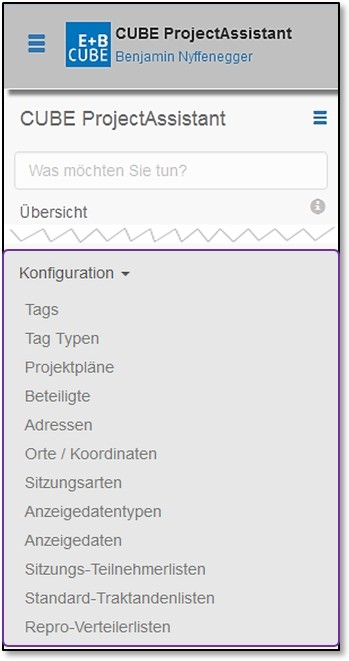
\includegraphics[width=1\linewidth]{../chapters/13_Konfigurationen/pictures/13_Menu_Konfiguration.jpg}
  \end{center}
  \vspace{-20pt}
  \caption{CUBE PA konfigurieren}
  \vspace{-10pt}
\end{wrapfigure}

Konfigurationen werden in der Regel durch einen Administrator oder sogenannte Poweruser, welche dazu speziell geschult wurden, vorgenommen. Entsprechend führt das Kapitel nicht Schritt für Schritt durch die Einstellungen. Im Zweifelsfall wird bei offenen Fragen oder Unsicherheiten empfohlen, den CUBE PA Support zu kontaktieren (siehe Kapitel \ref{bkm:Ref443502661}).

\vspace{\baselineskip}

Wählen Sie im Menü links den Punkt 'Konfiguration'. Es erscheinen die möglichen Unterpunkte, welche im Folgenden kurz erläutert werden.

\vspace{1.5cm} 

Benutzern, welchen die benötigten Rechte für die Konfiguration fehlen, wird dieser Punkt nicht angezeigt.

\vspace{3.5cm}  

\textbf{Übersicht über die Konfigurationsmöglichkeiten:}

\vspace{\baselineskip}

\begin{itemize}
\item
\textbf{Tags}: Hier werden Tags erfasst und den 'Tag Typen' zugeordnet. Tags werden z.B. im Dokumentenwesen verwendet, um Dokumente thematisch zu markieren und leichter wiederzufinden. Als Tags gelten z.B. auch die 'Projekte / Teilprojekte', welche an vielen Stellen in CUBE PA verwendet werden (z.B. Sitzungswesen,
Beschaffungswesen).
\item
\textbf{Tag Typen}: Gewünschte Tag Typen (Kategorien) werden hier erstellt, welchen dann die einzelnen Tags zugeordnet
werden können.
\item
\textbf{Projektpläne}: Es können mehrere Projektpläne (z.B. Detailterminprogramm) erstellt werden, welche bei der Funktion 'Importieren' (dann 'Termin Daten') separat ausgewählt und importiert werden können.
\item
\textbf{Beteiligte}: Hier werden Beteiligte angelegt, welche dann für verschiedene Zwecke in CUBE PA verwendet werden können. Beteiligte sind meistens Firmen, Gremien oder andere Organisationseinheiten. Je nach ihrer Funktion im Projekt können sie als 'Firma', 'Auftraggeber', 'Auftragnehmer', 'Gremium' usw. markiert werden. Diese Markierung beeinflusst, an welchen Stellen in CUBE PA die entsprechenden Beteiligten in den Auswahlboxen erscheinen.
\item
\textbf{Adressen}: Hier werden Adressen erfasst, die bei Sitzungen als Veranstaltungsort bzw. Ort der Protokollunterzeichnung ausgewählt werden können.
\item
\textbf{Orte / Koordinaten}: Diese Einträge beziehen sich auf projektbezogene 'Orte', z.B. Bahnübergänge, Bahnhöfe etc., welche mit Google-Maps verknüpft werden können. Diese vordefinierten Orte / Koordinaten erleichtern die Zuordnung von Koordinaten zu Dokumenten in der Dokumentenverwaltung. Die Verwendung ist jedoch freiwillig, es können auch beliebige, nicht im Voraus erfasste Koordinaten für die Zuweisung zu Dokumenten verwendet werden.
\item
\textbf{Sitzungsarten}: Hier werden die verschiedenen Sitzungsarten und standardmässige Verantwortliche verwaltet. Die Verwaltung der Zugriffsrechte zu den Sitzungen erfolgt in der aktuellen Version von CUBE PA ausschliesslich via die Benutzerverwaltung.
\item
\textbf{Anzeigedatentypen und Anzeigedaten}: Es ist möglich, wichtige Informationsdokumente, welche über wenige Klicks für die Benutzer zugänglich sein sollen, zu hinterlegen. Der Aufruf erfolgt über konfigurierbare Zusatzeinträge im Hauptmenü, die sog. Anzeigedatentypen. Für jeden Anzeigedatentyp kann festgelegt werden, in welcher Kategorie des Menüs der Eintrag erscheinen soll (z.B. im Sitzungswesen oder im Qualitätsmanagement). Die eigentlichen Dokumente werden
Anzeigedaten genannt. Es können mehrere Anzeigedaten zu einem Anzeigedatentypen zugeordnet werden. Zudem kann festgelegt werden, welche Person als Ansprechperson für das jeweilige Dokument zuständig ist. Es empfiehlt sich diese Funktionalität nur sehr sparsam einzusetzen, da ansonsten das Hauptmenü überladen werden könnte. Die Funktion wird beispielsweise für die Anzeige eines Gesamtterminprogramms verwendet, falls dieses nur in der Form einer Excel-Datei, nicht aber als MS Project-Datei gepflegt wird.
\item
\textbf{Sitzungs-Teilnehmerlisten}: Es können beliebige Teilnehmerlisten für Sitzungen zusammengestellt werden. Bei den ausgewählten Personen wird zudem definiert, ob sie auf der Verteilerliste stehen oder nicht. Diese Listen können anschliessend bei der Erstellung von Sitzungseinladungen ausgewählt werden.
\item
\textbf{Standard-Traktandenlisten}: Wiederkehrende, gleichbleibende Traktandenlisten können unter dieser Einstellung vordefiniert und später beim Erstellen einer Sitzung ausgewählt werden.
\item
\textbf{Repro-Verteilerlisten}: Personen, welche oft Pläne benötigen (Planlieferung in der Dokumentenablage) können hier in Verteilerlisten hinterlegt werden. In der Auswahl der Planlieferung können so anstelle der verschiedenen Personen diese vordefinierten Listen ausgewählt werden.
\end{itemize}

\vspace{\baselineskip}

Im Folgenden werden die verschiedenen Eingabemasken der oben beschriebenen Konfigurationspunkte kurz dokumentiert. Für weitere Detailinformationen oder sonstige Auskünfte wenden Sie sich bitte an den CUBE PA Support: {\color{red} cube.support@emchberger.ch}

\subsection{Tags}

Neue Tags werden hier erstellt, können angezeigt oder bearbeitet werden.

\begin{figure}[H]
\center{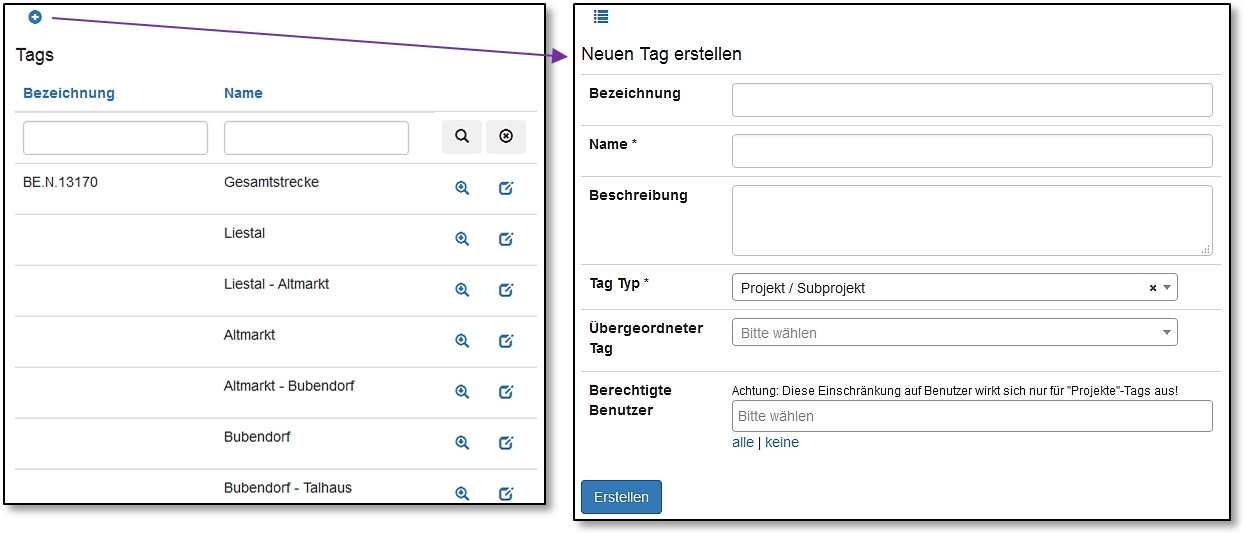
\includegraphics[width=1\linewidth]{../chapters/13_Konfigurationen/pictures/13-1_TagsHinzufuegen.jpg}}
\caption{Neue Tags erstellen}
% \label{fig:speciation}
\end{figure}

Die 'Bezeichnung' wird momentan nur für die Projekt-/Teilprojekt-Tags genutzt. Hier kann die Projektnummer eingetragen werden.

\vspace{\baselineskip}

Der 'Name' (Pflichtfeld) wird überall in CUBE PA für den entsprechenden Tag verwendet. Erfasste Tags müssen einem Tag Typen (siehe Kapitel \ref{bkm:Ref444100222}) zugewiesen werden.

\vspace{\baselineskip}

Es ist möglich, Tags hierarchisch zu erfassen. Dazu ist in den jeweils untergeordneten Tags das Feld 'Übergeordneter Tag' auszufüllen. Zu einem Tag können mehrere untergeordnete Tags definiert werden.

\vspace{\baselineskip}

Beachten Sie, dass sich die Auswahl von berechtigten Benutzern nur auf 'Projekte'-Tags auswirkt (siehe Hinweis).

\subsection{Tag Typen}
\label{bkm:Ref444100222}
Da Tags ein sehr universelles Hilfsmittel in CUBE PA darstellen, ist es möglich, verschiedene Kategorien von Tags, die sogenannten Tag Typen zu definieren. \newline

Damit ist es möglich, Dokumente nach verschiedenen Kriterien mit Tags zu versehen. Beispielsweise sind dies die Dokumentenart oder das Fachgebiet. Auch die Kategorie 'Projekt / Teilprojekt' ist als Tag Type hinterlegt, wobei der Haken bei 'Ist Projekt' gesetzt ist. Damit wird erreicht, dass die Tags dieser Kategorie überall dort ausgewählt werden können, wo die Zuweisung zu einem Teilprojekt erwünscht ist (z.B. bei Sitzungen oder Beschaffungen). \newline

Tag Typen, welche für die Kategorisierung von Dokumenten verwendet werden sollen, werden mit dem Haken bei 'Ist Dokumententag' versehen. Die Anzeigereihenfolge der Tag Typen kann mittels Eingabe einer Zahl im Feld 'Position' festgelegt werden. Die Reihenfolge erfolgt aufsteigend.

\begin{figure}[H]
\center{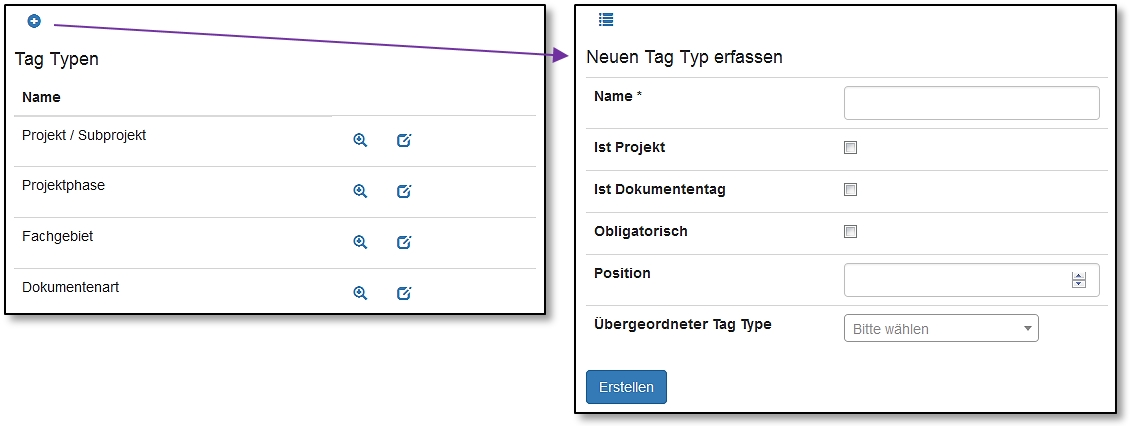
\includegraphics[width=1\linewidth]{../chapters/13_Konfigurationen/pictures/13-2_TagTypenHinzufuegen.jpg}}
\caption{Neuer Tag Typ erfassen}
% \label{fig:speciation}
\end{figure}

\subsection{Projektpläne}

Es können mehrere Projektpläne (z.B. Detailterminprogramm, Terminprogramme für Teilprojekte) erstellt werden, für welche mit der Funktion 'Importieren' (dann  'Termin Daten') separate Datensätze eingelesen werden können.

\begin{figure}[H]
\center{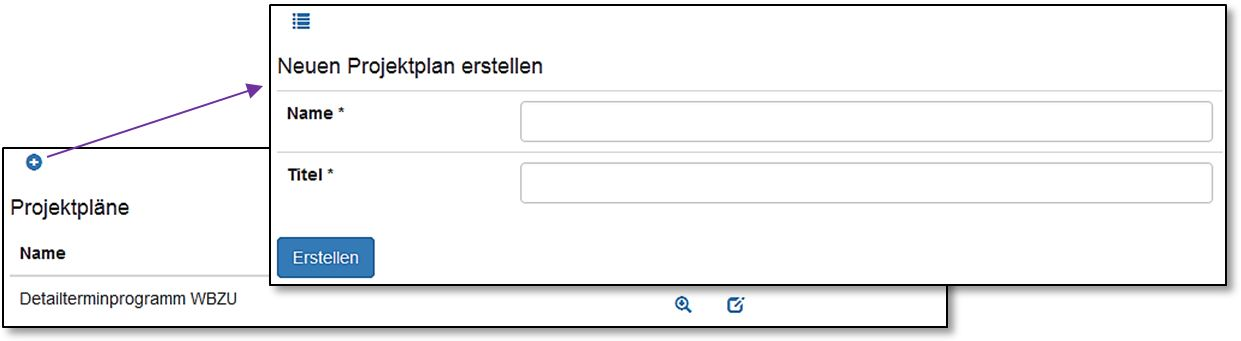
\includegraphics[width=1\linewidth]{../chapters/13_Konfigurationen/pictures/13-3_ProjektplaeneHinzufuegen.jpg}}
\caption{Neuen Projektplan erstellen}
% \label{fig:speciation}
\end{figure}

Alle erfassten Projektpläne werden hier aufgelistet. Sie können in der Detailansicht betrachtet oder geändert werden. Unter diesem Konfigurationspunkt werden ebenfalls neue Einträge erstellt.

\subsection{Beteiligte}
\label{bkm:Ref2018071602}

\begin{wrapfigure}[13]{r}{6cm}
\vspace{-45pt}
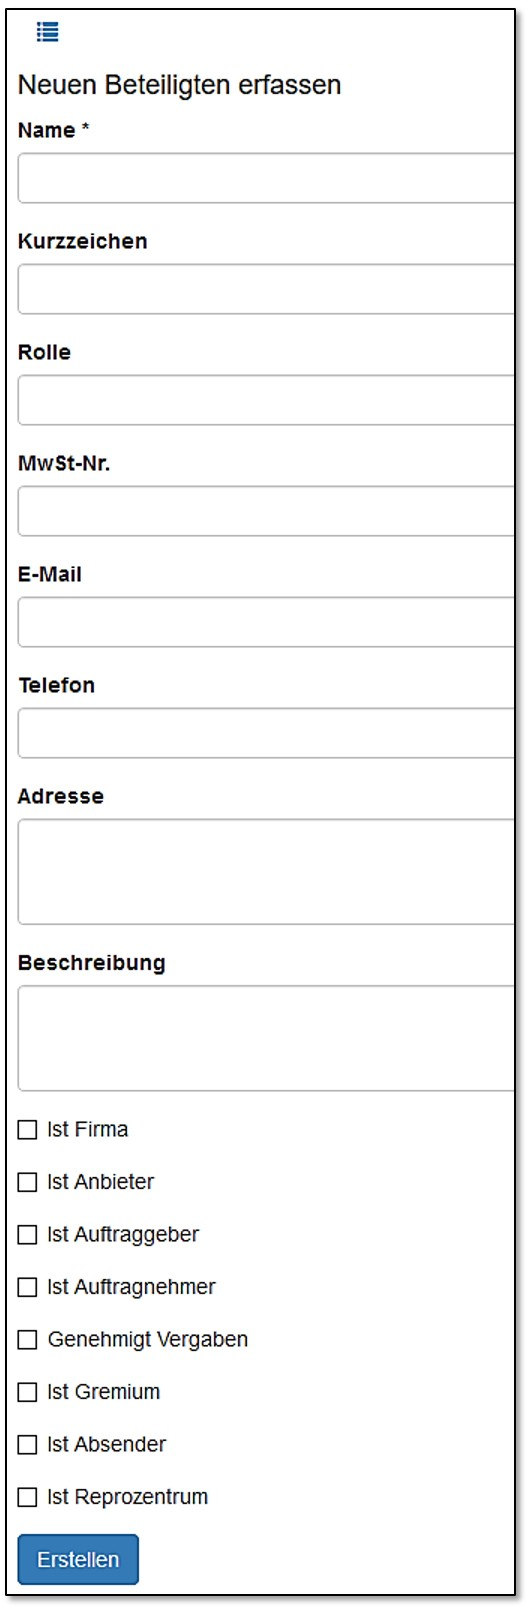
\includegraphics[height=150mm]{../chapters/13_Konfigurationen/pictures/konf_BeteiligteErfassen.jpg}
% \caption{Status ändern}
\end{wrapfigure}

Hier werden bei einem Projekt beteiligte Personen angelegt, welche dann für verschiedene 'Rollen' definiert werden können.

\begin{center}
\hspace{-15pt}   
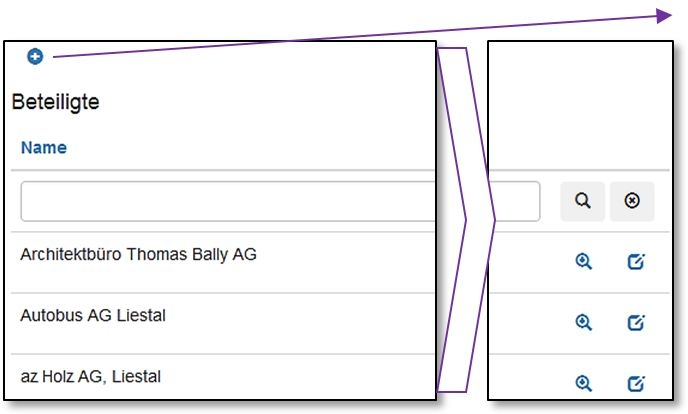
\includegraphics[width=.9\linewidth]{../chapters/13_Konfigurationen/pictures/13-4_Beteiligte.jpg}
\end{center}

Das Feld 'Rolle' bietet per Freitext die Rolle eines Beteiligten innerhalb eines Projektes zu beschreiben. 

\vspace{\baselineskip}

Die Checkboxen unten 'Ist Firma', 'Ist Arbeitgeber' etc. ermöglichen die Auswahl als wen Beteiligte in Bereichen von CUBE PA referenziert werden können. Wurde beispielsweise '[x] Ist Firma' markiert, wird jeweils beim Auswahl-/Dropdown-Feld 'Firma' dieser Beteiligte zur Auswahl angezeigt.\\

\textbf{Ist Reprozentrum:} Wie ein Reprozentrum eingerichtet wird, ist in Kapitel \ref{bkm:Ref2018071601} ersichtlich.

\vspace{\baselineskip}
\vspace{\baselineskip}
\vspace{\baselineskip}


\subsection{Adressen}

Adressen sind in aller Regel Sitzungszimmer. Es können jedoch auch Standorte (ohne Sitzungszimmerfunktion) erfasst werden. Entsprechend ist bei 'Ist Sitzungszimmer' beim Erfassen einer Adresse das Häkchen zu setzen oder leer zu lassen.

\begin{figure}[H]
\center{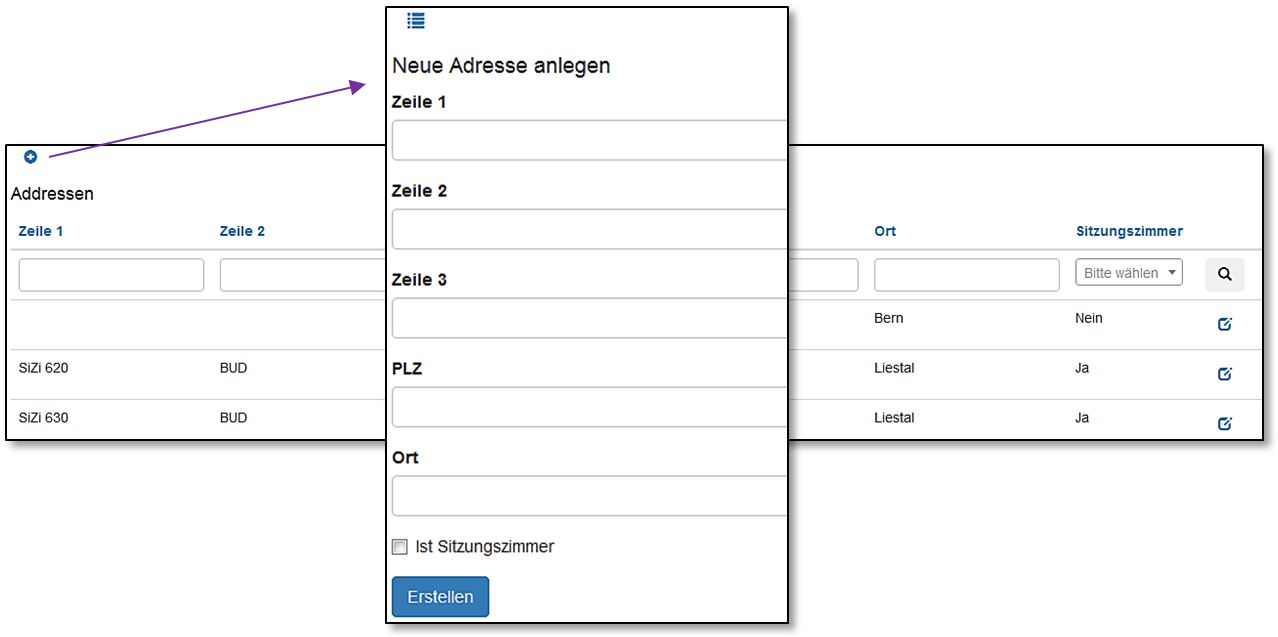
\includegraphics[width=1\linewidth]{../chapters/13_Konfigurationen/pictures/13-5_AdresseHinzufuegen.jpg}}
\caption{Neue Adresse anlegen}
% \label{fig:speciation}
\end{figure}

\subsection{Orte / Koordinaten}

Diese Einträge beziehen sich auf projektbezogene 'Orte', z.B. Bahnübergänge, Bahnhöfe etc., welche mit Google-Maps verknüpft werden können. Bei Klick auf die 'Nadel' wird auf Google-Maps die Position beschriftet angezeigt.

\begin{figure}[H]
\center{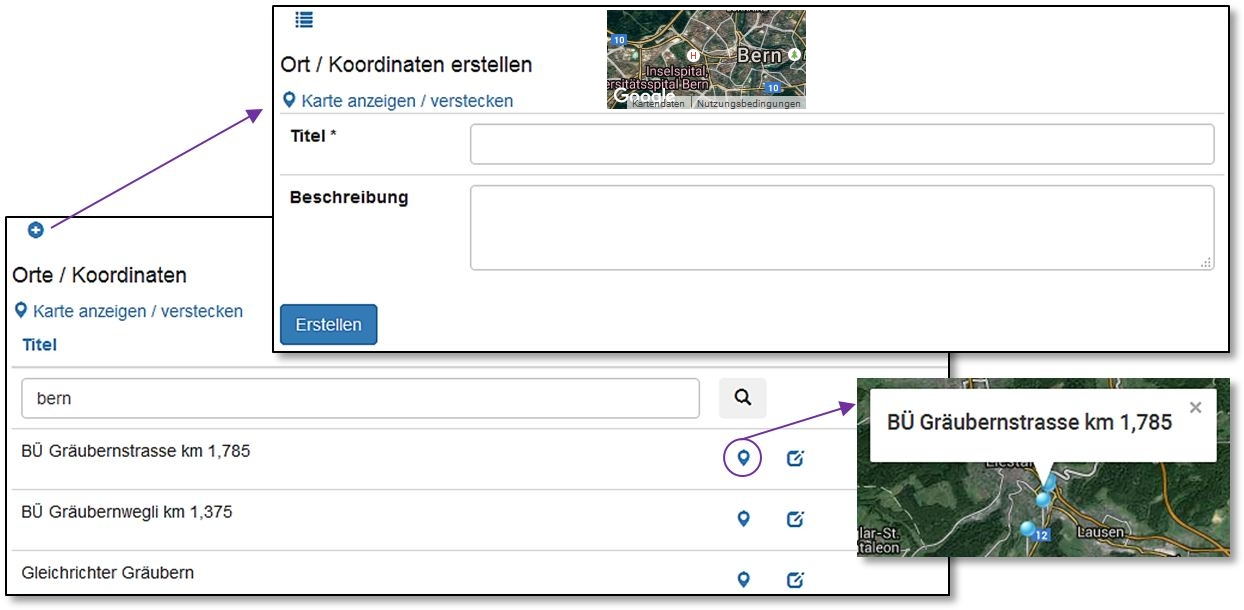
\includegraphics[width=1\linewidth]{../chapters/13_Konfigurationen/pictures/13-6_KoordinatenHinzufuegen.jpg}}
\caption{Ort / Koordinaten erstellen}
% \label{fig:speciation}
\end{figure}

\clearpage
\subsection{Sitzungsarten}

Hier werden die verschiedenen Sitzungsarten und die dazu berechtigten Benutzer erfasst.

\vspace{\baselineskip}


Für eine Sitzung kann der 'Vorsitz' und 'Stv. Vorsitz' vordefiniert und bei Bedarf später wieder angepasst
werden.

\begin{figure}[H]
\center{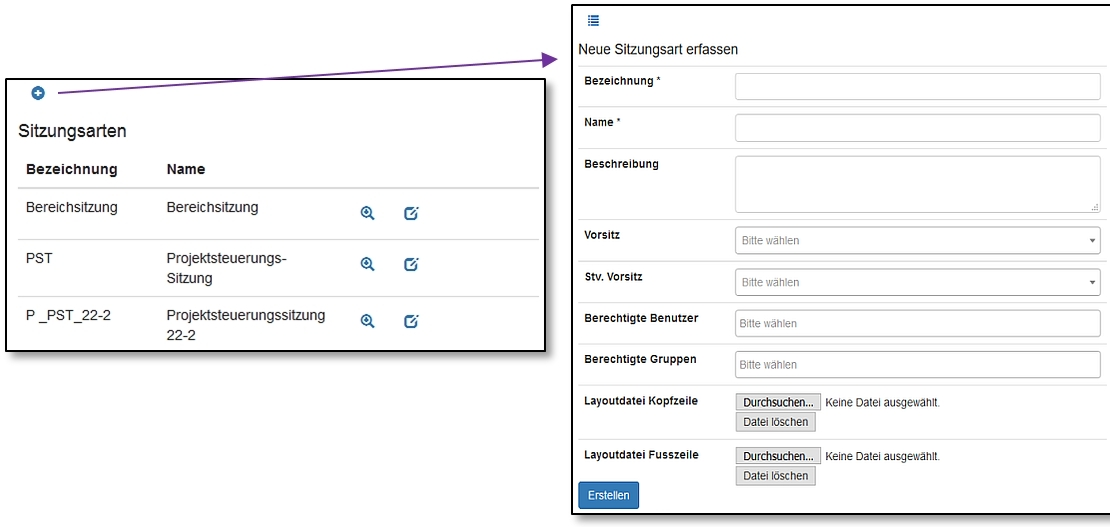
\includegraphics[width=1\linewidth]{../chapters/13_Konfigurationen/pictures/13-7_SitzungsartHinzufuegen.jpg}}
\caption{Neue Sitzungsart erfassen}
% \label{fig:speciation}
\end{figure}

\subsection{Anzeigedatentypen und Anzeigedaten}

Es ist möglich wichtige Informationsdokumente, welche über wenige Klicks für die Benutzer zugänglich sein sollen, zu hinterlegen. Der Aufruf erfolgt über konfigurierbare Zusatzeinträge im Hauptmenü, die sog. Anzeigedatentypen. Für jeden Anzeigedatentyp kann festgelegt werden, in welcher Kategorie des Menüs der Eintrag erscheinen soll (z.B. im Sitzungswesen oder im Qualitätsmanagement). Die eigentlichen Dokumente werden Anzeigedaten genannt. Es können mehrere Anzeigedaten zu einem Anzeigedatentypen zugeordnet werden. Zudem kann festgelegt werden, welche Person als Ansprechperson für das jeweilige Dokument zuständig ist. Es empfiehlt sich diese Funktionalität nur sehr sparsam einzusetzen, da ansonsten das Hauptmenü überladen werden könnte. Die Funktion wird beispielsweise für die Anzeige eines Gesamtterminprogramms verwendet, falls dieses nur in der Form einer Excel-Datei, nicht aber als MS Project-Datei gepflegt wird.

\vspace{\baselineskip}

Der Name eines Anzeigedatentyps ist möglichst prägnant und kurz zu halten. Entsprechend des Eintrages (Name) wird dieser im Menü unter der ausgewählten Kategorie angezeigt. Also sind mehrere Worte oder ein Satz zu vermeiden.

\begin{figure}[H]
\center{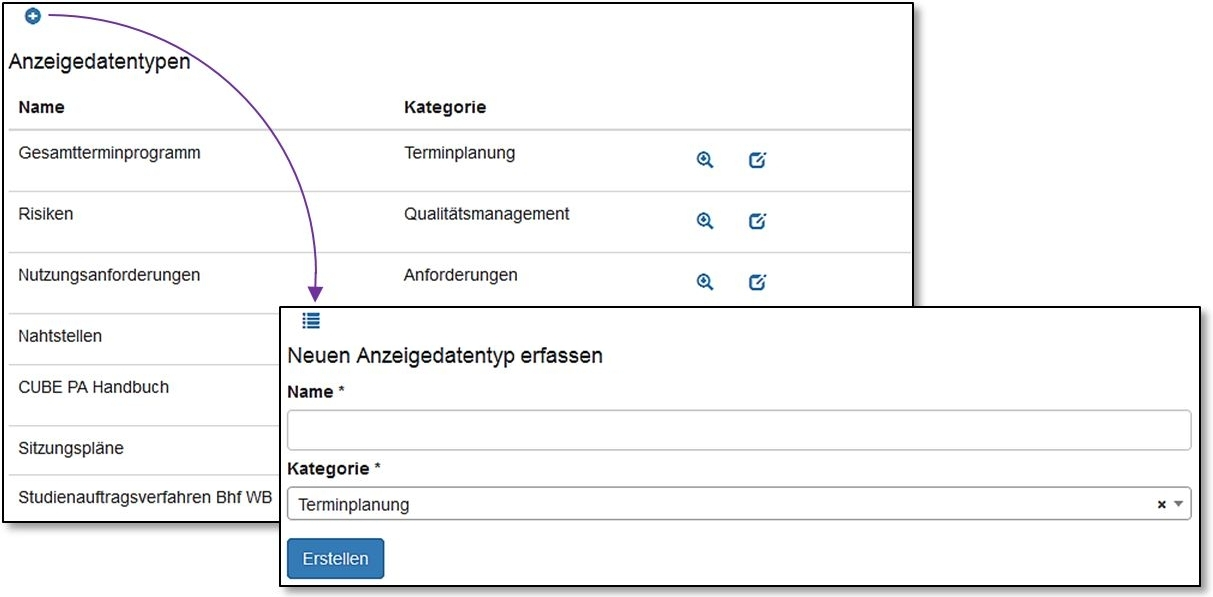
\includegraphics[width=1\linewidth]{../chapters/13_Konfigurationen/pictures/13-8_AnzeigetypenErfassen.jpg}}
\caption{Neue Anzeigedatentypen erfassen}
% \label{fig:speciation}
\end{figure}

\begin{figure}[H]
\center{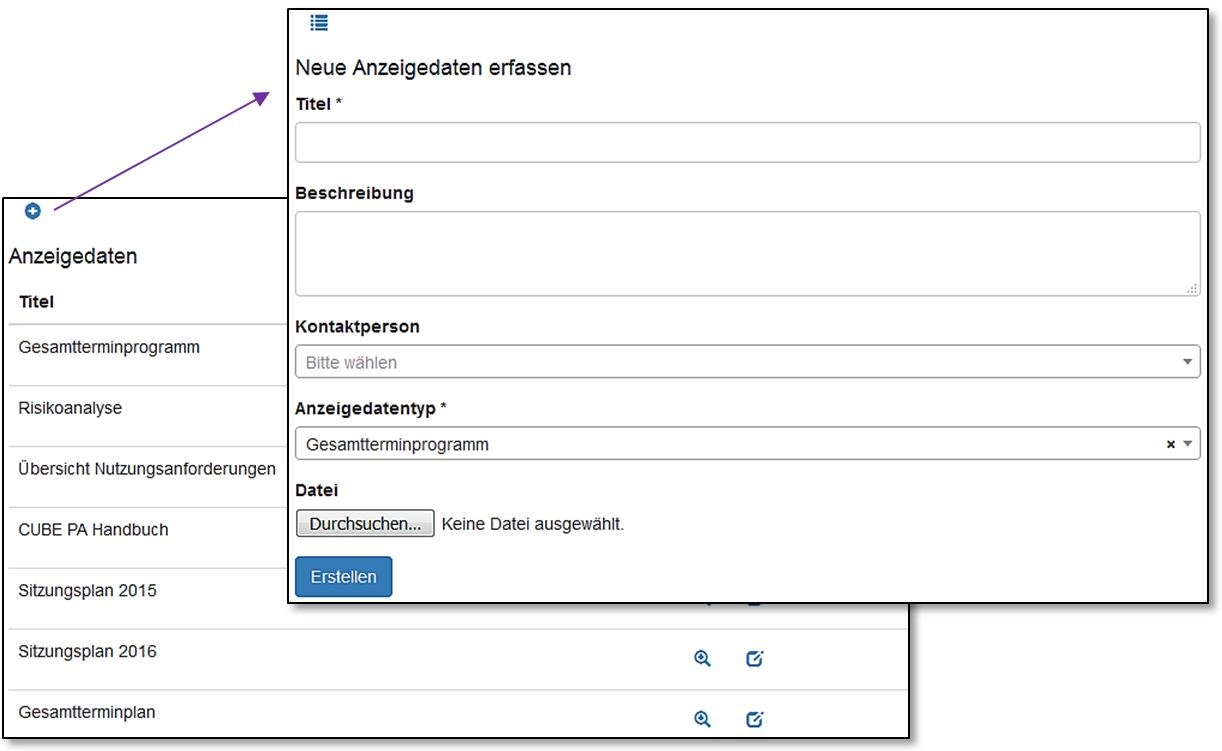
\includegraphics[width=1\linewidth]{../chapters/13_Konfigurationen/pictures/13-8_AnzeigedatenErfassen.jpg}}
\caption{Neue Anzeigedaten erfassen}
% \label{fig:speciation}
\end{figure}

% \small{Übersicht und Eingabemöglichkeiten für die Anzeigedatentypen und Anzeigedaten.}

\clearpage
\subsection{Sitzungs-Teilnehmerlisten}

Es können beliebige Teilnehmerlisten für Sitzungen zusammengestellt werden. Bei den ausgewählten Personen wird zudem definiert, ob sie auf der Verteilerliste stehen oder nicht.

\begin{figure}[H]
\center{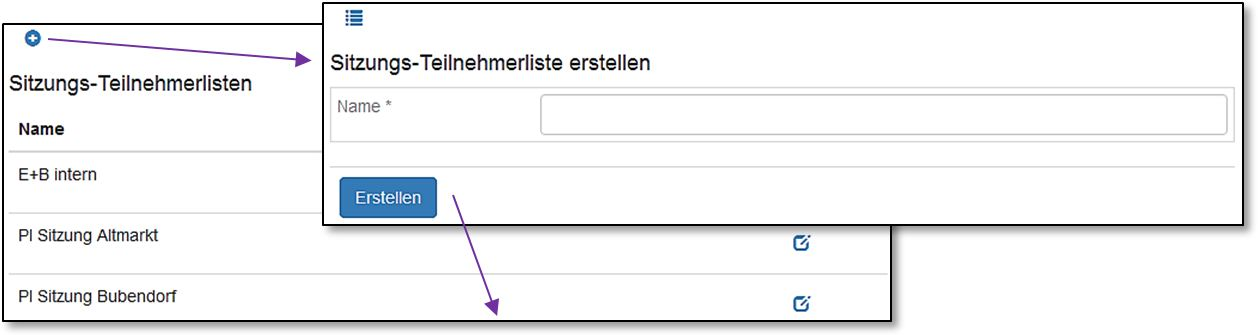
\includegraphics[width=1\linewidth]{../chapters/13_Konfigurationen/pictures/13-9_SitzungsteilnehmerlistenErstellen.jpg}}
% \caption{Sitzungs-Teilnehmerlisten erstellen}
% \label{fig:speciation}
\end{figure}

\begin{figure}[H]
\vspace{-25pt}
\center{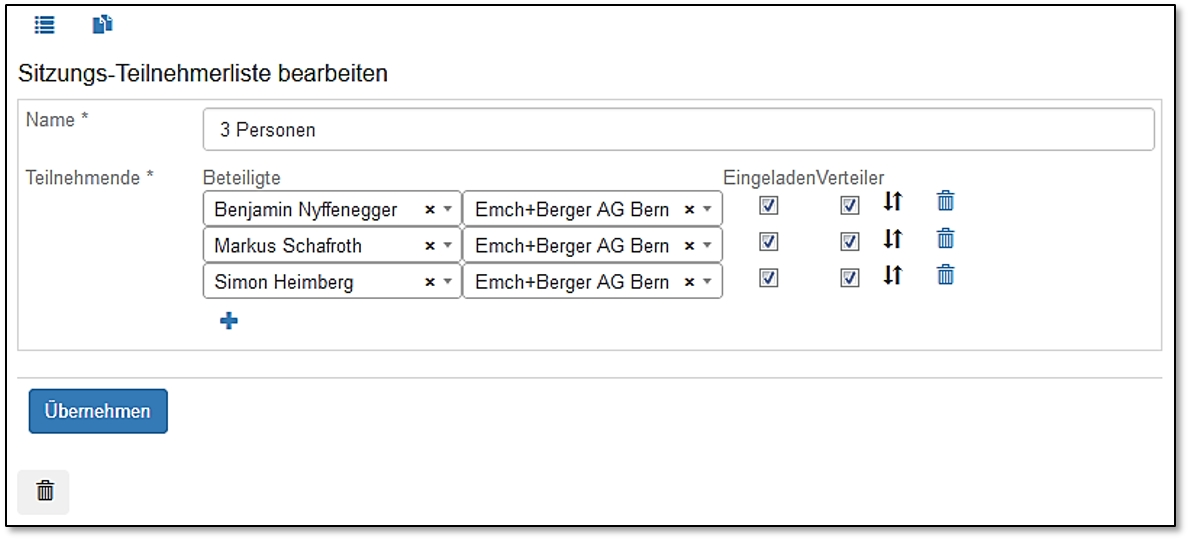
\includegraphics[width=0.75\linewidth]{../chapters/13_Konfigurationen/pictures/13-9_SitzungsteilnehmerlistenBearbeiten.jpg}}
\caption{Sitzungs-Teilnehmerlisten erstellen und bearbeiten}
% \label{fig:speciation}
\end{figure}

Erst nach Klick auf 'Erstellen' einer neuen Liste wird es möglich, Mitglieder hinzuzufügen. Mitglieder können in der Reihenfolge verschoben und wieder gelöscht werden. Hier können Sie zudem definieren, ob es sich bei den Teilnehmenden um an Sitzungen 'Eingeladene' handelt oder ob sie nur auf der Protokollverteilerliste stehen sollen. Wird ersteres angewählt, können Sie bei der Protokollführung jeweils auswählen, ob die Eingeladenen an Sitzungen 'anwesend' oder 'entschuldigt' sind. Zuunterst im Fenster kann eine erstellte Sitzungs-Teilnehmerliste gelöscht werden.

\vspace{\baselineskip}

\textbf{Standardteilnehmerlisten kopieren:}\\
Sie haben mittels dem 'Kopiersymbol' 
\includegraphics[height=12pt]{/Icons/kopieren.jpg} die Möglichkeit, Standardteilnehmerlisten zu kopieren. Kicken Sie auf das Symbol, öffnet sich der kopierte Datensatz, welcher Sie nun anpassen können. Der kopierte Datensatz enthält vor und nach dem Namen drei Sternen, also bspw. ***Sitzungsteilnehmer***.

\clearpage
\subsection{Standard-Traktandenlisten}

Wiederkehrende, gleichbleibende Traktandenlisten können unter dieser Einstellung vordefiniert und später beim Erstellen einer Sitzung ausgewählt werden.

\begin{figure}[H]
\center{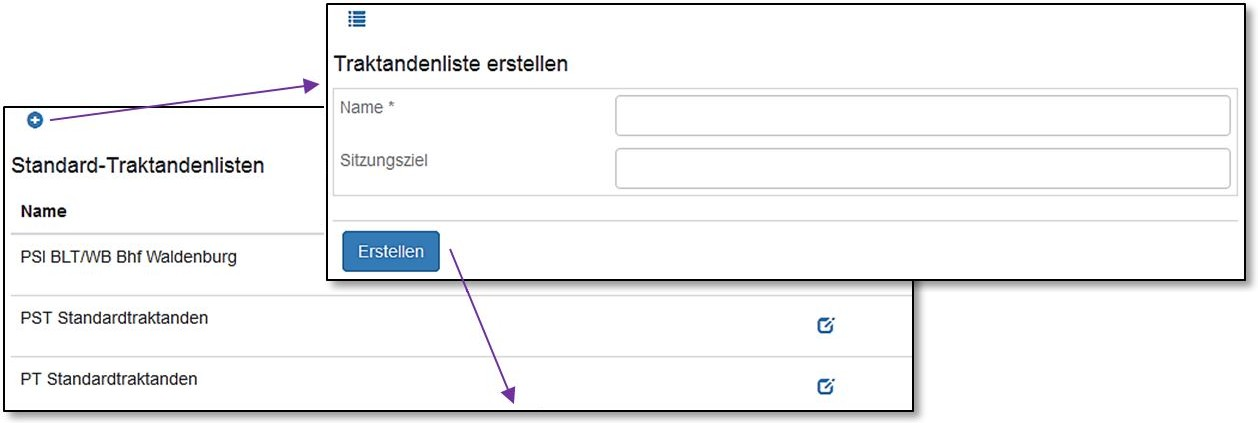
\includegraphics[width=1\linewidth]{../chapters/13_Konfigurationen/pictures/13-10_TraktandenlistenErstellen.jpg}}
\caption{Traktandenlisten erstellen}
% \label{fig:speciation}
\end{figure}

\begin{wrapfigure}[14]{r}{9cm}
\vspace{-15pt}
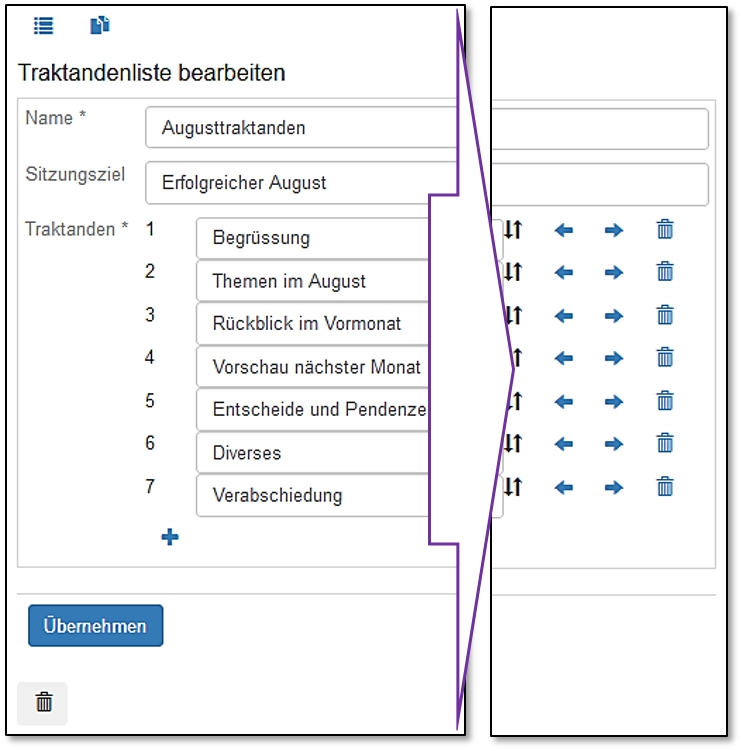
\includegraphics[height=85mm]{../chapters/13_Konfigurationen/pictures/13-10_TraktandenlistenBearbeiten.jpg}
% \caption{Status ändern}
\end{wrapfigure}

Erst nach dem 'Erstellen' einer neuen Traktandenliste erscheint die Möglichkeit, Traktanden zu erfassen oder zu bearbeiten. Neue Traktanden können in der Reihenfolge wie auch in der Gliederung (1, 2, 3 oder 2, 2.1, 3 etc.) verschoben werden. Einzelne Traktanden wie auch eine ganze Liste können hier gelöscht werden. Wie bei den Standard-Teilnehmerlisten kann eine Traktandenliste mittels dem 'Kopiersymbol' 
\includegraphics[height=12pt]{/Icons/kopieren.jpg} kopiert werden. Der kopierte Datensatz ist an den drei Sternen vor und nach dem Namen erkennbar (z.B. ***Traktandenliste***). 

\subsection{Repro-Konfigurationen}

\subsubsection{Repro-Verteilerlisten}

Es können Verteilerlisten erstellt werden, für Personen welche wiederkehrend Ausdrucke erhalten sollen.

\begin{figure}[H]
\center{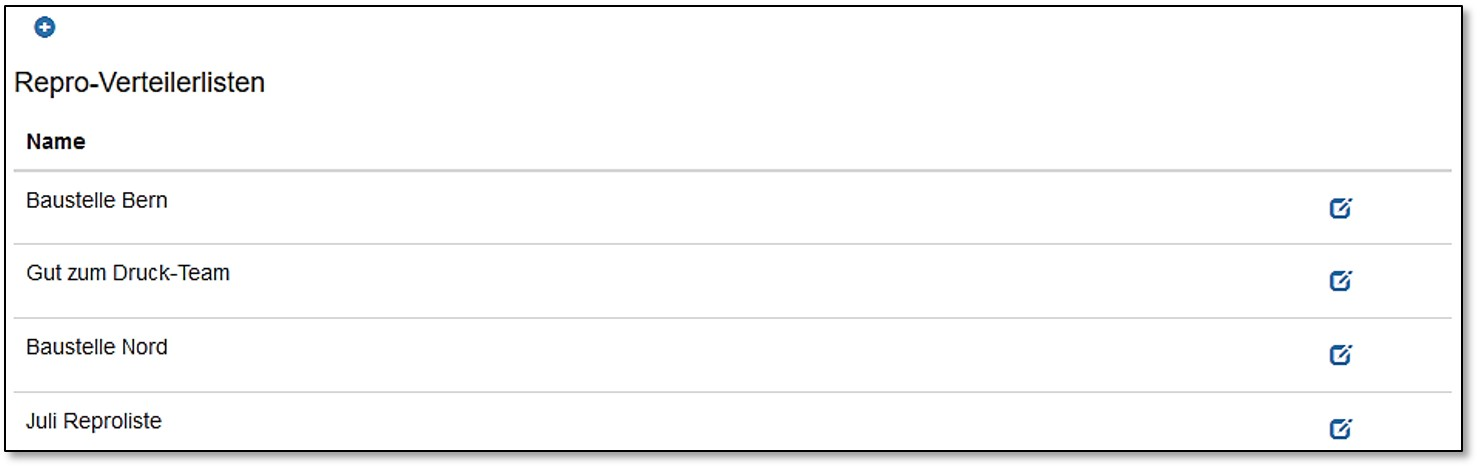
\includegraphics[width=1\linewidth]{../chapters/13_Konfigurationen/pictures/konf_ReproVListe_Uebersicht.jpg}}
\caption{Repro-Verteilerlisten in der Übersicht}
% \label{fig:speciation}
\end{figure}

Die Listen enthalten die gewünschten Personen, sowie die gängigen Einstellungen (Anzahl Exemplare, ausgedruckte Dokumente, elektronisch zugestellte Dokumente). Einzelne Empfänger wie auch ganze Listen können hier auch wieder gelöscht werden:

\begin{figure}[H]
\center{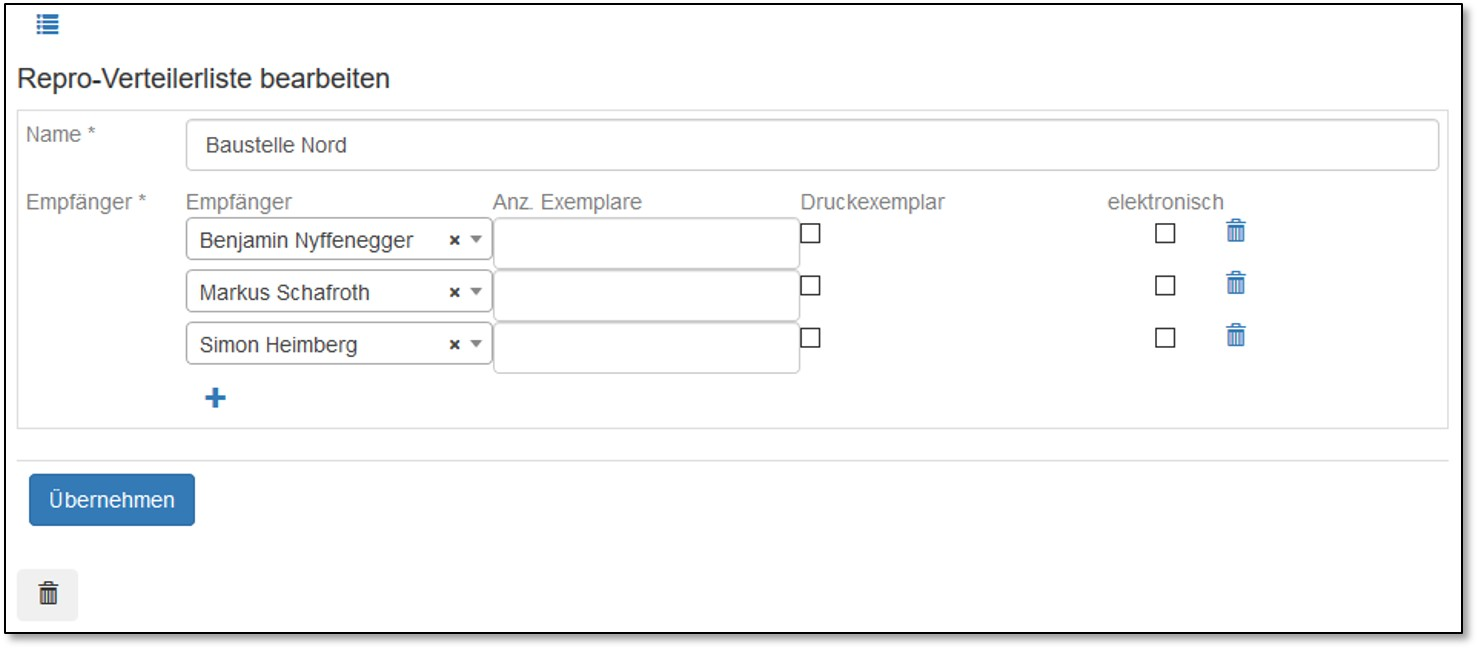
\includegraphics[width=1\linewidth]{../chapters/13_Konfigurationen/pictures/konf_ReproVListe_edit.jpg}}
\caption{Repro-Verteilerlisten im Bearbeitungsmodus}
% \label{fig:speciation}
\end{figure}

\subsubsection{Reprozentren einrichten}
\label{bkm:Ref2018071601}

Um Pläne an ein Reprozentrum senden zu können, muss dieses zuerst angelegt werden:

\begin{enumerate}
\item Legen Sie im Menü 'Konfigurationen' unter 'Beteiligte' das Reprozentrum an. Siehe dazu auch Kapitel \ref{bkm:Ref2018071602}. Setzten Sie ein Häkchen bei 'Ist Reprozentrum'
\item Wiederholen Sie obigen Schritt für sämtliche Reprozentren, welche beim Versand / Druck von Dokumenten ausgewählt werden können.
\item Erstellen Sie im Menü 'Benutzerverwaltung' unter 'Gruppen' eine neue Gruppe, welche sämtliche Druckzentren (Punkt 1 und 2) enthält.
\end{enumerate}

\textbf{Hinweis:} Bei der Planlieferung in der Dokumentenablage werden nicht die Gruppen, sondern die erstellten Druckzentren (Beteiligte) ausgewählt.




